\documentclass[aspectratio=169]{beamer}


\usepackage[T1]{fontenc}
\usepackage[ngerman]{babel}

\usepackage[duration=30]{pdfpcnotes}    % https://github.com/cebe/pdfpc-latex-notes 	
\usepackage{amsmath, amssymb, amstext}
\usepackage{stmaryrd}
\usepackage{graphicx}
\usepackage{xcolor}
\usepackage{tikz}
\usepackage{appendixnumberbeamer}
\usepackage{enumerate}
\usepackage{listings}
\usepackage{lstautogobble}
\usepackage{multicol}
\usepackage{lmodern}
\usepackage{lipsum}
\usepackage{marvosym}

\usetheme{metropolis}

\metroset{%
    block=fill
}

\newcommand{\code}[1]{\colorbox{lightgray}{\vphantom{|}\texttt{#1}}}
\newcommand{\cmd}[1]{\code{\$ #1}}
\newcommand{\gitcmd}[1]{\cmd{git #1}}

\titlegraphic{%
    
\includegraphics[height=1cm]{rust-logo}
}

\title{Raytracing}
\subtitle{Rust Proseminar}

\author[Sami Shalayel, Daniel Freiermuth, Carl Schwan]{%
    Autoren: Sami Shalayel, Daniel Freiermuth, Carl Schwan}

\institute{Universität des Saarlandes}
\date{\today}

\begin{document}

\maketitle

\begin{frame}{Überblick}
    \setbeamertemplate{section in toc}[sections numbered]
    \tableofcontents[hideallsubsections]
\end{frame}

\section{Projektstruktur}
\begin{frame}[fragile]{Primitive Objekte: Interceptable Trait}
    Wir können alles rendern, was den ,,Interceptable''-Trait implementiert : \\

    Dieser gibt an, ob, wo und wie das Objekt von einem Lichtstrahl getroffen wird.

    \pause
    Beispiele für ,,Interceptable'':
    \begin{itemize}[<+->]
        \item Kugeln
        \item Ebenen
        \item Dreiecke
        \item Beschleunigungsstrukturen
    \end{itemize}

\end{frame}


\begin{frame}[fragile]{Shaders: Shader Trait}
    \pnote{
        Interceptable returned halt alles,\\
        was der shader so zum rendern braucht (dh auch Distanz zum Objekt, Winkel zur Oberfläche,  ...)
    }
    Jeder Shader liefert eine Farbe für einen Lichtstrahl-Objekt-Schnitt.

    \pause
    Wir haben folgende Shader implementiert :

    \begin{itemize}[<+->]
        \item Monochrome shader
        \item Chess shader
        \item Diffuse shader
        \item Mirror shader
        \item Specular shader
        \item Multiplicative shader
        \item Additive shader
    \end{itemize}
\end{frame}
\begin{frame}[fragile]{Phong Shader}
    \begin{lstlisting}
pub fn get_phong(color: Vector3<f64>)
-> Box<Shader> {
    let diffuse_shader: Box<Shader> =
Box::new(DiffuseShader { color: color });
    let specular_shader = SpecularShader
{ alpha: 10.0 };
    let ambient_shader: Box<Shader> =
    Box::new(MonochromeShader {
        color: Vector3::new(0.1, 0.1, 0.1),
    });
    return 0.5 * diffuse_shader + specular_shader
+ 0.5 * ambient_shader;
}
    \end{lstlisting}
\end{frame}
\begin{frame}{Shaders: Shader Trait}
    \begin{columns}[t]
        \column{.5\textwidth}
        \centering
        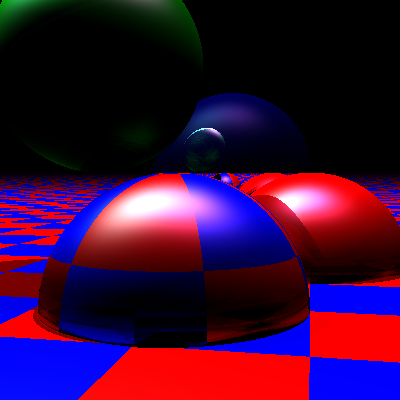
\includegraphics[height=3cm]{example-true-ambiant} \\
        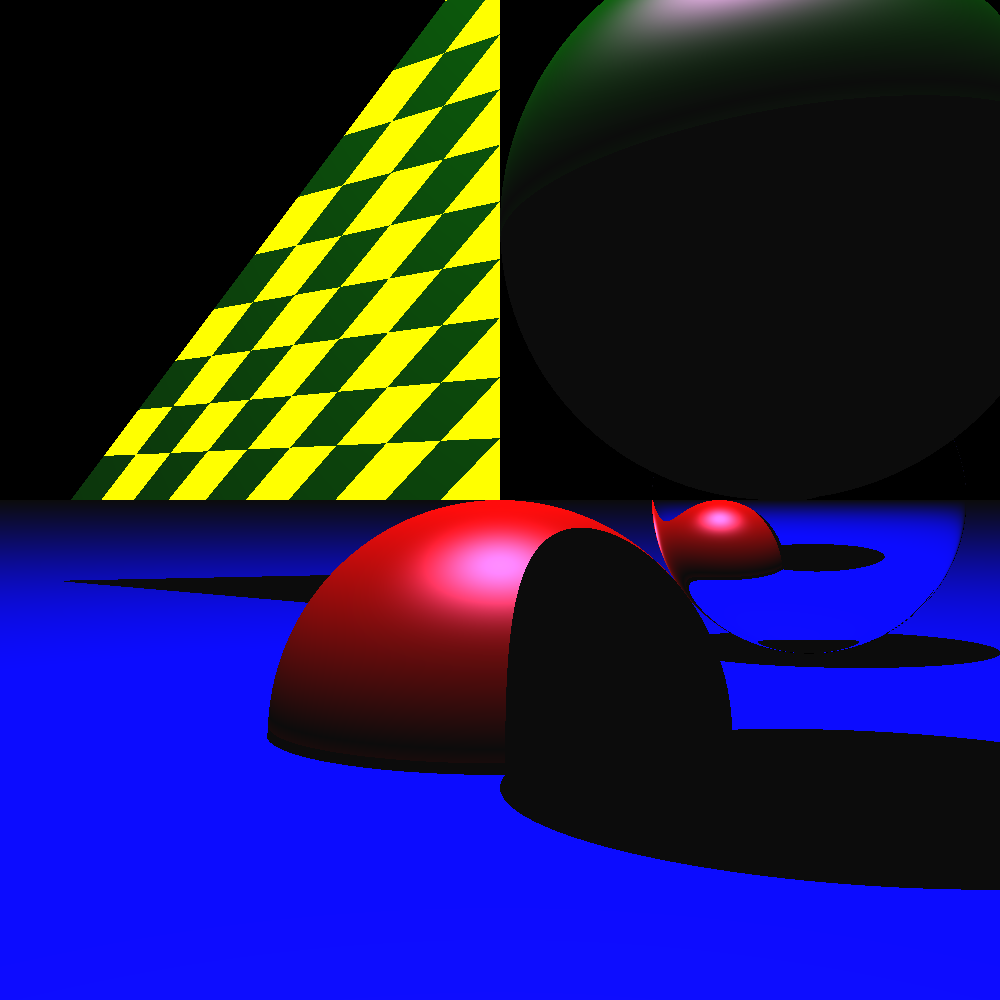
\includegraphics[height=3cm]{example-mirror}
        \column{.5\textwidth}
        \centering
        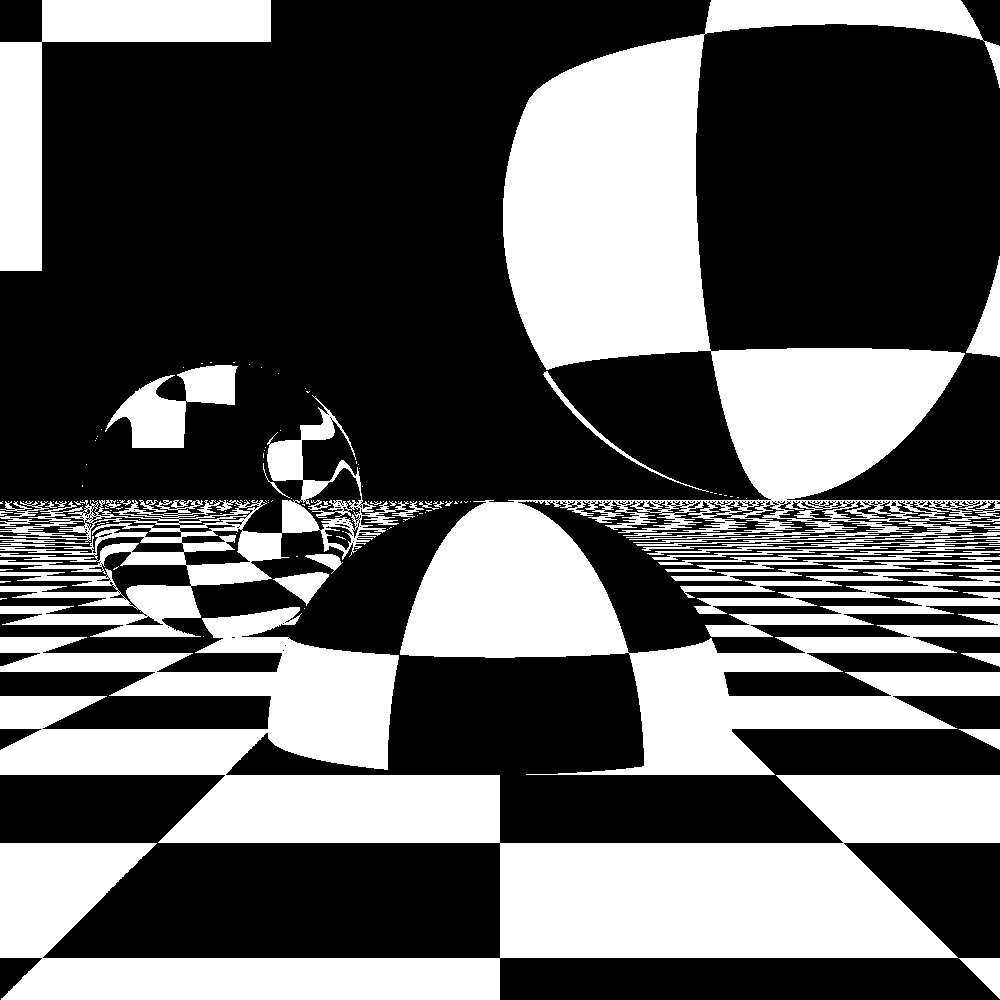
\includegraphics[height=3cm]{example-mirror2}
    \end{columns}
\end{frame}
\begin{frame}[fragile]{Camera Trait}
    \begin{lstlisting}
pub trait Camera {
    fn render(&self, world: &World) -> DynamicImage;
}
    \end{lstlisting}
\end{frame}
\begin{frame}{Cameras: Implemtierung}
    \begin{itemize}[<+->]
        \item Equilinear Camera
        \item Equirectangular Camera
    \end{itemize}
\end{frame}
\begin{frame}{Wavefront Parser}
    \begin{itemize}[<+->]
        \item Wavefront Obj parser
        \item Wavefront Mtl parser
    \end{itemize}
    Benutzt die wavefront\_obj crate
\end{frame}
\begin{frame}{Wavefront Parser}
    
\includegraphics[height=3cm]{example-duck}
\end{frame}
\begin{frame}{Storage und World}
    TODO Explanation storage
\end{frame}
\section{Rust in unsere Projekt}
\begin{frame}[fragile]{Operator overload}
    \begin{lstlisting}
impl Add for Box<Shader> {
    type Output = Box<Shader>;
    fn add(self, other: Box<Shader>) -> Box<Shader> {
        Box::new(AdditiveShader {
            shader1: self,
            shader2: other,
        })
    }
}
    \end{lstlisting}
\end{frame}
\begin{frame}{Nalgebra und std::f64}
    TODO
\end{frame}
\begin{frame}{Error Handling}
    TODO
\end{frame}
\section{Störend in Rust}
\begin{frame}{Störend in Rust}
    \begin{itemize}[<+->]
        \item Mehr Arbeit durch Borrow-Checker/Lifetimes
        \item Rayon
    \end{itemize}
\end{frame}
\section{Lessons learned}
\begin{frame}{Lesons learned}
    \begin{itemize}[<+->]
        \item Reference in Struct -> Lifetime
        \item Serde
        \item ...
    \end{itemize}
\end{frame}

\begin{frame}[standout]
\centering
\Huge Vielen Dank für eure Aufmerksamkeit!

\end{frame}

\end{document}
